% Options for packages loaded elsewhere
\PassOptionsToPackage{unicode}{hyperref}
\PassOptionsToPackage{hyphens}{url}
%
\documentclass[
]{article}
\usepackage{amsmath,amssymb}
\usepackage{iftex}
\ifPDFTeX
  \usepackage[T1]{fontenc}
  \usepackage[utf8]{inputenc}
  \usepackage{textcomp} % provide euro and other symbols
\else % if luatex or xetex
  \usepackage{unicode-math} % this also loads fontspec
  \defaultfontfeatures{Scale=MatchLowercase}
  \defaultfontfeatures[\rmfamily]{Ligatures=TeX,Scale=1}
\fi
\usepackage{lmodern}
\ifPDFTeX\else
  % xetex/luatex font selection
\fi
% Use upquote if available, for straight quotes in verbatim environments
\IfFileExists{upquote.sty}{\usepackage{upquote}}{}
\IfFileExists{microtype.sty}{% use microtype if available
  \usepackage[]{microtype}
  \UseMicrotypeSet[protrusion]{basicmath} % disable protrusion for tt fonts
}{}
\makeatletter
\@ifundefined{KOMAClassName}{% if non-KOMA class
  \IfFileExists{parskip.sty}{%
    \usepackage{parskip}
  }{% else
    \setlength{\parindent}{0pt}
    \setlength{\parskip}{6pt plus 2pt minus 1pt}}
}{% if KOMA class
  \KOMAoptions{parskip=half}}
\makeatother
\usepackage{xcolor}
\usepackage[margin=1in]{geometry}
\usepackage{color}
\usepackage{fancyvrb}
\newcommand{\VerbBar}{|}
\newcommand{\VERB}{\Verb[commandchars=\\\{\}]}
\DefineVerbatimEnvironment{Highlighting}{Verbatim}{commandchars=\\\{\}}
% Add ',fontsize=\small' for more characters per line
\usepackage{framed}
\definecolor{shadecolor}{RGB}{248,248,248}
\newenvironment{Shaded}{\begin{snugshade}}{\end{snugshade}}
\newcommand{\AlertTok}[1]{\textcolor[rgb]{0.94,0.16,0.16}{#1}}
\newcommand{\AnnotationTok}[1]{\textcolor[rgb]{0.56,0.35,0.01}{\textbf{\textit{#1}}}}
\newcommand{\AttributeTok}[1]{\textcolor[rgb]{0.13,0.29,0.53}{#1}}
\newcommand{\BaseNTok}[1]{\textcolor[rgb]{0.00,0.00,0.81}{#1}}
\newcommand{\BuiltInTok}[1]{#1}
\newcommand{\CharTok}[1]{\textcolor[rgb]{0.31,0.60,0.02}{#1}}
\newcommand{\CommentTok}[1]{\textcolor[rgb]{0.56,0.35,0.01}{\textit{#1}}}
\newcommand{\CommentVarTok}[1]{\textcolor[rgb]{0.56,0.35,0.01}{\textbf{\textit{#1}}}}
\newcommand{\ConstantTok}[1]{\textcolor[rgb]{0.56,0.35,0.01}{#1}}
\newcommand{\ControlFlowTok}[1]{\textcolor[rgb]{0.13,0.29,0.53}{\textbf{#1}}}
\newcommand{\DataTypeTok}[1]{\textcolor[rgb]{0.13,0.29,0.53}{#1}}
\newcommand{\DecValTok}[1]{\textcolor[rgb]{0.00,0.00,0.81}{#1}}
\newcommand{\DocumentationTok}[1]{\textcolor[rgb]{0.56,0.35,0.01}{\textbf{\textit{#1}}}}
\newcommand{\ErrorTok}[1]{\textcolor[rgb]{0.64,0.00,0.00}{\textbf{#1}}}
\newcommand{\ExtensionTok}[1]{#1}
\newcommand{\FloatTok}[1]{\textcolor[rgb]{0.00,0.00,0.81}{#1}}
\newcommand{\FunctionTok}[1]{\textcolor[rgb]{0.13,0.29,0.53}{\textbf{#1}}}
\newcommand{\ImportTok}[1]{#1}
\newcommand{\InformationTok}[1]{\textcolor[rgb]{0.56,0.35,0.01}{\textbf{\textit{#1}}}}
\newcommand{\KeywordTok}[1]{\textcolor[rgb]{0.13,0.29,0.53}{\textbf{#1}}}
\newcommand{\NormalTok}[1]{#1}
\newcommand{\OperatorTok}[1]{\textcolor[rgb]{0.81,0.36,0.00}{\textbf{#1}}}
\newcommand{\OtherTok}[1]{\textcolor[rgb]{0.56,0.35,0.01}{#1}}
\newcommand{\PreprocessorTok}[1]{\textcolor[rgb]{0.56,0.35,0.01}{\textit{#1}}}
\newcommand{\RegionMarkerTok}[1]{#1}
\newcommand{\SpecialCharTok}[1]{\textcolor[rgb]{0.81,0.36,0.00}{\textbf{#1}}}
\newcommand{\SpecialStringTok}[1]{\textcolor[rgb]{0.31,0.60,0.02}{#1}}
\newcommand{\StringTok}[1]{\textcolor[rgb]{0.31,0.60,0.02}{#1}}
\newcommand{\VariableTok}[1]{\textcolor[rgb]{0.00,0.00,0.00}{#1}}
\newcommand{\VerbatimStringTok}[1]{\textcolor[rgb]{0.31,0.60,0.02}{#1}}
\newcommand{\WarningTok}[1]{\textcolor[rgb]{0.56,0.35,0.01}{\textbf{\textit{#1}}}}
\usepackage{graphicx}
\makeatletter
\def\maxwidth{\ifdim\Gin@nat@width>\linewidth\linewidth\else\Gin@nat@width\fi}
\def\maxheight{\ifdim\Gin@nat@height>\textheight\textheight\else\Gin@nat@height\fi}
\makeatother
% Scale images if necessary, so that they will not overflow the page
% margins by default, and it is still possible to overwrite the defaults
% using explicit options in \includegraphics[width, height, ...]{}
\setkeys{Gin}{width=\maxwidth,height=\maxheight,keepaspectratio}
% Set default figure placement to htbp
\makeatletter
\def\fps@figure{htbp}
\makeatother
\setlength{\emergencystretch}{3em} % prevent overfull lines
\providecommand{\tightlist}{%
  \setlength{\itemsep}{0pt}\setlength{\parskip}{0pt}}
\setcounter{secnumdepth}{-\maxdimen} % remove section numbering
\ifLuaTeX
  \usepackage{selnolig}  % disable illegal ligatures
\fi
\IfFileExists{bookmark.sty}{\usepackage{bookmark}}{\usepackage{hyperref}}
\IfFileExists{xurl.sty}{\usepackage{xurl}}{} % add URL line breaks if available
\urlstyle{same}
\hypersetup{
  pdftitle={Práctica 2: Limpieza y análisis de datos},
  pdfauthor={Maider Dorronsoro, Flavia Felletti},
  hidelinks,
  pdfcreator={LaTeX via pandoc}}

\title{Práctica 2: Limpieza y análisis de datos}
\author{Maider Dorronsoro, Flavia Felletti}
\date{2023-06-14}

\begin{document}
\maketitle

{
\setcounter{tocdepth}{2}
\tableofcontents
}
\newpage{}

\hypertarget{descripciuxf3n-del-dataset.}{%
\section{1 Descripción del dataset.}\label{descripciuxf3n-del-dataset.}}

El dataset seleccionado son datos relativos a pacientes de diferentes
países, en concreto a pacientes con alguna enfermedad cardiovascular.
Según los datos de la World Health Organization (WHO), las enfermedades
cardiovasculares son la principal causa de muerte en el mundo. Se ha
calculado que cada año al rededor de 17.9 millones de personas pierden
su vida por alguna enfermedad cardiovascular.Además, un tercio de ellos,
son personas menores a 70 años, lo cual provoca una muerte temprana.Por
ello, creemos importante e interesante analizar esta problemática.

Al fin y al cabo, en este proyecto se va a analizar/detectar los
factores que más aumentan la probabilidad de padecer de enfermedades
cardiovasculares El dataset ha sido obtenido de esta fuente:
\url{https://www.kaggle.com/datasets/rashikrahmanpritom/heart-attack-analysis-prediction-dataset}

\begin{Shaded}
\begin{Highlighting}[]
\NormalTok{df}\OtherTok{\textless{}{-}}\FunctionTok{read.csv}\NormalTok{(}\StringTok{"heart.csv"}\NormalTok{)}
\NormalTok{df}\SpecialCharTok{$}\NormalTok{sex }\OtherTok{\textless{}{-}} \FunctionTok{as.character}\NormalTok{(df}\SpecialCharTok{$}\NormalTok{sex)}
\end{Highlighting}
\end{Shaded}

A continuación, se procede a hacer un pequeño análisis del dataset:

\begin{Shaded}
\begin{Highlighting}[]
\CommentTok{\# visualizo las dimensiones del dataset:}
\NormalTok{dimdat }\OtherTok{\textless{}{-}} \FunctionTok{dim}\NormalTok{(df)}
\NormalTok{dimdat}
\end{Highlighting}
\end{Shaded}

\begin{verbatim}
## [1] 303  14
\end{verbatim}

Tenemos un conjunto de datos con 303 registros y 14 variables a
analizar, de las cuales solo vamos a describir las que nos interesan en
este análisis.

\begin{itemize}
  \item Age:Edad de los pacientes
  \item Sex:Género pacientes [0: F, 1: M]
  \item trtbps: Resting blood pressure- Presión arterial en reposo [mm Hg]
  \item chol: Colesterol [mm/dl]
  \item restecg: Resultados del electrocardiograma en reposo [0: Normal, 1: con anormalidad de la onda ST-T, 2: muestra hipertrofia ventricular izquierda probable o definitiva según los criterios de Estes].
  \item thalachh: Frecuencia cardíaca máxima alcanzada [Valor numérico entre 71 y 202]
  \item output: Enfermedad cardiaca [1: tiene enfermedad cardíaca, 0: no tiene enfermedad cardíaca]
\end{itemize}

A continuación un resumen estadístico de las diferentes variables a
analizar:

\begin{Shaded}
\begin{Highlighting}[]
\FunctionTok{summary}\NormalTok{(df)}
\end{Highlighting}
\end{Shaded}

\begin{verbatim}
##       age            sex                  cp            trtbps     
##  Min.   :29.00   Length:303         Min.   :0.000   Min.   : 94.0  
##  1st Qu.:47.50   Class :character   1st Qu.:0.000   1st Qu.:120.0  
##  Median :55.00   Mode  :character   Median :1.000   Median :130.0  
##  Mean   :54.37                      Mean   :0.967   Mean   :131.6  
##  3rd Qu.:61.00                      3rd Qu.:2.000   3rd Qu.:140.0  
##  Max.   :77.00                      Max.   :3.000   Max.   :200.0  
##       chol            fbs            restecg          thalachh    
##  Min.   :126.0   Min.   :0.0000   Min.   :0.0000   Min.   : 71.0  
##  1st Qu.:211.0   1st Qu.:0.0000   1st Qu.:0.0000   1st Qu.:133.5  
##  Median :240.0   Median :0.0000   Median :1.0000   Median :153.0  
##  Mean   :246.3   Mean   :0.1485   Mean   :0.5281   Mean   :149.6  
##  3rd Qu.:274.5   3rd Qu.:0.0000   3rd Qu.:1.0000   3rd Qu.:166.0  
##  Max.   :564.0   Max.   :1.0000   Max.   :2.0000   Max.   :202.0  
##       exng           oldpeak          slp             caa        
##  Min.   :0.0000   Min.   :0.00   Min.   :0.000   Min.   :0.0000  
##  1st Qu.:0.0000   1st Qu.:0.00   1st Qu.:1.000   1st Qu.:0.0000  
##  Median :0.0000   Median :0.80   Median :1.000   Median :0.0000  
##  Mean   :0.3267   Mean   :1.04   Mean   :1.399   Mean   :0.7294  
##  3rd Qu.:1.0000   3rd Qu.:1.60   3rd Qu.:2.000   3rd Qu.:1.0000  
##  Max.   :1.0000   Max.   :6.20   Max.   :2.000   Max.   :4.0000  
##      thall           output      
##  Min.   :0.000   Min.   :0.0000  
##  1st Qu.:2.000   1st Qu.:0.0000  
##  Median :2.000   Median :1.0000  
##  Mean   :2.314   Mean   :0.5446  
##  3rd Qu.:3.000   3rd Qu.:1.0000  
##  Max.   :3.000   Max.   :1.0000
\end{verbatim}

\begin{center}\rule{0.5\linewidth}{0.5pt}\end{center}

\hypertarget{integraciuxf3n-y-selecciuxf3n-de-los-datos-de-interuxe9s-a-analizar.}{%
\section{2 Integración y selección de los datos de interés a
analizar.}\label{integraciuxf3n-y-selecciuxf3n-de-los-datos-de-interuxe9s-a-analizar.}}

En este proyecto se quiere analizar la realidad de las enfermedades
cardiovasculares de las personas en relación a las variables
seleccionadas.Como unicamente nos interesan las mencioandas, se hace una
subselección de estas.

\begin{Shaded}
\begin{Highlighting}[]
\NormalTok{df }\OtherTok{\textless{}{-}} \FunctionTok{select}\NormalTok{ (df,}\StringTok{\textquotesingle{}age\textquotesingle{}}\NormalTok{,}\StringTok{\textquotesingle{}sex\textquotesingle{}}\NormalTok{, }\StringTok{\textquotesingle{}chol\textquotesingle{}}\NormalTok{,}\StringTok{\textquotesingle{}restecg\textquotesingle{}}\NormalTok{,}\StringTok{\textquotesingle{}trtbps\textquotesingle{}}\NormalTok{,}\StringTok{\textquotesingle{}thalachh\textquotesingle{}}\NormalTok{,}\StringTok{\textquotesingle{}output\textquotesingle{}}\NormalTok{)}
\NormalTok{df}\SpecialCharTok{$}\NormalTok{sex }\OtherTok{\textless{}{-}} \FunctionTok{ifelse}\NormalTok{(df}\SpecialCharTok{$}\NormalTok{sex}\SpecialCharTok{==}\StringTok{\textquotesingle{}0\textquotesingle{}}\NormalTok{,}\StringTok{\textquotesingle{}F\textquotesingle{}}\NormalTok{,}\StringTok{\textquotesingle{}M\textquotesingle{}}\NormalTok{)}
\FunctionTok{head}\NormalTok{(df)}
\end{Highlighting}
\end{Shaded}

\begin{verbatim}
##   age sex chol restecg trtbps thalachh output
## 1  63   M  233       0    145      150      1
## 2  37   M  250       1    130      187      1
## 3  41   F  204       0    130      172      1
## 4  56   M  236       1    120      178      1
## 5  57   F  354       1    120      163      1
## 6  57   M  192       1    140      148      1
\end{verbatim}

\begin{center}\rule{0.5\linewidth}{0.5pt}\end{center}

\hypertarget{limpieza-de-los-datos.}{%
\section{3 Limpieza de los datos.}\label{limpieza-de-los-datos.}}

\hypertarget{los-datos-contienen-ceros-o-elementos-vacuxedos-gestiona-cada-uno-de-estos-casos.}{%
\subsection{3.1. ¿Los datos contienen ceros o elementos vacíos? Gestiona
cada uno de estos
casos.}\label{los-datos-contienen-ceros-o-elementos-vacuxedos-gestiona-cada-uno-de-estos-casos.}}

A continuación se procede a analizar la existencia de valores perdidos
NA, NULL o blancos:

\begin{Shaded}
\begin{Highlighting}[]
\CommentTok{\# averiguo si el dataset contiene valores NA ("not available")}
\FunctionTok{any}\NormalTok{(}\FunctionTok{is.na}\NormalTok{(df))}
\end{Highlighting}
\end{Shaded}

\begin{verbatim}
## [1] FALSE
\end{verbatim}

\begin{Shaded}
\begin{Highlighting}[]
\CommentTok{\# averiguo si hay valores NULL}
\FunctionTok{any}\NormalTok{(}\FunctionTok{is.null}\NormalTok{(df))}
\end{Highlighting}
\end{Shaded}

\begin{verbatim}
## [1] FALSE
\end{verbatim}

\begin{Shaded}
\begin{Highlighting}[]
\CommentTok{\# averiguo si hay valores blancos}
\FunctionTok{any}\NormalTok{(df }\SpecialCharTok{==} \StringTok{""}\NormalTok{)}
\end{Highlighting}
\end{Shaded}

\begin{verbatim}
## [1] FALSE
\end{verbatim}

Tal y como se puede observar no hay registros incompletos, por lo que no
se van a tratar.

\hypertarget{identifica-y-gestiona-los-valores-extremos}{%
\subsection{3.2. Identifica y gestiona los valores
extremos}\label{identifica-y-gestiona-los-valores-extremos}}

\textbf{Diagrama de cajas de la variable Cholesterol}

\begin{Shaded}
\begin{Highlighting}[]
\FunctionTok{boxplot}\NormalTok{(df}\SpecialCharTok{$}\NormalTok{chol,}
  \AttributeTok{ylab =} \StringTok{"Cholesterol levels"}\NormalTok{,}
  \AttributeTok{col =} \StringTok{"red3"}
\NormalTok{)}
\end{Highlighting}
\end{Shaded}

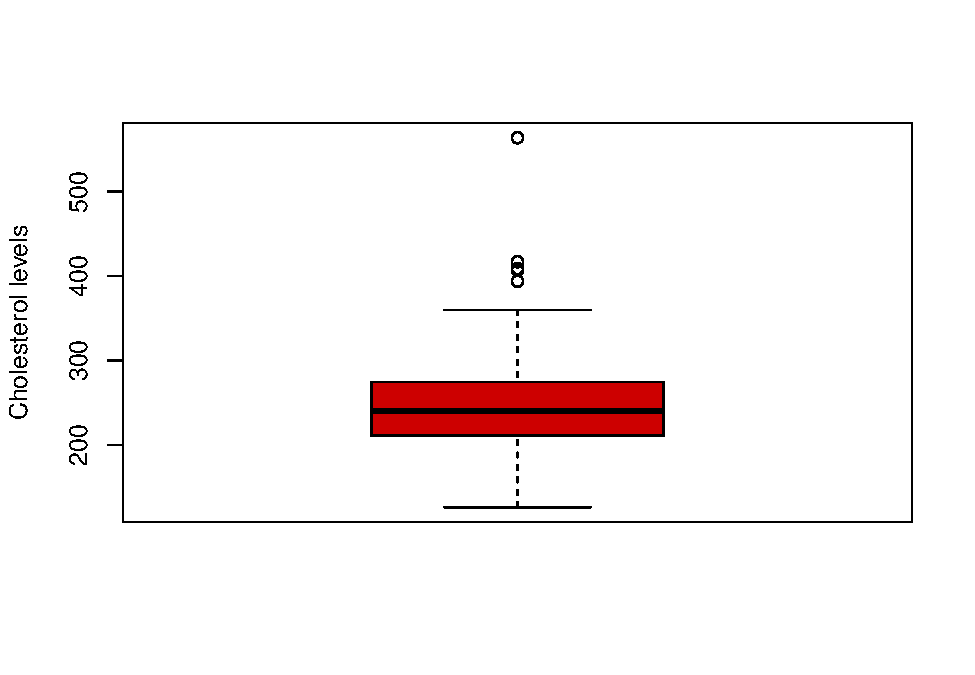
\includegraphics{PRA2_files/figure-latex/unnamed-chunk-5-1.pdf}

\textbf{Histograma de la variable Cholesterol}

\begin{Shaded}
\begin{Highlighting}[]
\FunctionTok{hist}\NormalTok{(df}\SpecialCharTok{$}\NormalTok{chol, }\AttributeTok{xlab=}\StringTok{"Cholesterol"}\NormalTok{,}
     \AttributeTok{main=}\StringTok{"Cholesterol Distribution"}\NormalTok{, }\AttributeTok{col=}\StringTok{"red3"}\NormalTok{)}
\end{Highlighting}
\end{Shaded}

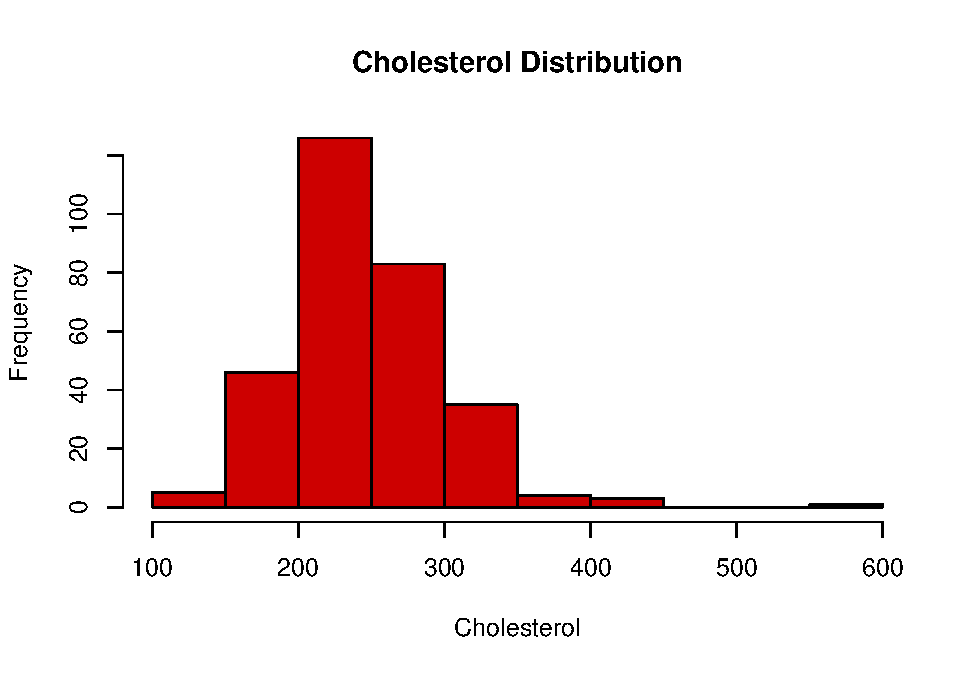
\includegraphics{PRA2_files/figure-latex/unnamed-chunk-6-1.pdf} Se puede
observar que existen valores de colesteról que superan los 400 mm/dl.
Esto no tiene porqué ser resultado de un error; de hecho, el colesteról
tan alto podría ser causa de una enfermedad cardiaca grave.\footnote{según
  este artículo en la sección ``health'' de CNN, hay condiciones
  genéticas que pueden provocar niveles de hasta 600 mg/dL
  \url{http://edition.cnn.com/2009/HEALTH/11/24/moh.healthmag.cholesterol.surprises/index.html\#}:\textasciitilde:text=But\%20for\%20some\%20families\%2C\%20it's,heart\%20attacks\%20early\%20in\%20life.}

Otros casos de incosistencisa o datos incoherentes podrían ser los
valores de restecg (presión arterial en en reposo) y Chol (colesterol)
iguales a 0.

A continuación se analiza la cantidad de resgistros que tienen
colesterol igual a 0 y/o presión arterial en reposo igual a 0.

\begin{Shaded}
\begin{Highlighting}[]
\CommentTok{\# Cholesterol equal zero}
\StringTok{"Cholesterol:"}
\end{Highlighting}
\end{Shaded}

\begin{verbatim}
## [1] "Cholesterol:"
\end{verbatim}

\begin{Shaded}
\begin{Highlighting}[]
\FunctionTok{sum}\NormalTok{(df}\SpecialCharTok{$}\NormalTok{chol }\SpecialCharTok{==} \DecValTok{0}\NormalTok{)}
\end{Highlighting}
\end{Shaded}

\begin{verbatim}
## [1] 0
\end{verbatim}

\begin{Shaded}
\begin{Highlighting}[]
\CommentTok{\# RestingBP equal zero}
\StringTok{"RestingBP:"}
\end{Highlighting}
\end{Shaded}

\begin{verbatim}
## [1] "RestingBP:"
\end{verbatim}

\begin{Shaded}
\begin{Highlighting}[]
\FunctionTok{sum}\NormalTok{(df}\SpecialCharTok{$}\NormalTok{trtbps }\SpecialCharTok{==} \DecValTok{0}\NormalTok{)}
\end{Highlighting}
\end{Shaded}

\begin{verbatim}
## [1] 0
\end{verbatim}

Contamos el número de observaciones que tienen colesteról inferior a 40
mg/dL, que equivale a niveles muy bajos de colesteról, aunque
probables.\footnote{Según el artículo:
  \url{https://www.mayoclinic.org/diseases-conditions/high-blood-cholesterol/expert-answers/cholesterol-level/faq-20057952}}

\begin{Shaded}
\begin{Highlighting}[]
\FunctionTok{sum}\NormalTok{(df}\SpecialCharTok{$}\NormalTok{chol }\SpecialCharTok{\textless{}} \DecValTok{40}\NormalTok{)}
\end{Highlighting}
\end{Shaded}

\begin{verbatim}
## [1] 0
\end{verbatim}

Se eliminarán del conjunto de datos las observaciones que tienen niveles
de colesterol o de presión cardíaca en reposo iguales a cero y se vuelve
a visualizar el resúmen estadistico.

\begin{Shaded}
\begin{Highlighting}[]
\CommentTok{\# creates a new dataset deleting Cholesterol = 0 and RestingBP = 0 from}
\CommentTok{\# the original dataset}
\NormalTok{dff }\OtherTok{\textless{}{-}}\NormalTok{ df[(df}\SpecialCharTok{$}\NormalTok{chol }\SpecialCharTok{!=} \DecValTok{0} \SpecialCharTok{\&}\NormalTok{ df}\SpecialCharTok{$}\NormalTok{restecg }\SpecialCharTok{!=} \DecValTok{0}\NormalTok{),]}

\CommentTok{\# visualizes summary}
\FunctionTok{summary}\NormalTok{(dff)}
\end{Highlighting}
\end{Shaded}

\begin{verbatim}
##       age            sex                 chol          restecg     
##  Min.   :34.00   Length:156         Min.   :126.0   Min.   :1.000  
##  1st Qu.:45.00   Class :character   1st Qu.:204.0   1st Qu.:1.000  
##  Median :54.00   Mode  :character   Median :232.0   Median :1.000  
##  Mean   :53.12                      Mean   :237.9   Mean   :1.026  
##  3rd Qu.:60.00                      3rd Qu.:266.2   3rd Qu.:1.000  
##  Max.   :76.00                      Max.   :354.0   Max.   :2.000  
##      trtbps         thalachh         output      
##  Min.   : 94.0   Min.   : 71.0   Min.   :0.0000  
##  1st Qu.:120.0   1st Qu.:138.8   1st Qu.:0.0000  
##  Median :128.5   Median :157.5   Median :1.0000  
##  Mean   :129.4   Mean   :151.3   Mean   :0.6218  
##  3rd Qu.:140.0   3rd Qu.:169.0   3rd Qu.:1.0000  
##  Max.   :180.0   Max.   :194.0   Max.   :1.0000
\end{verbatim}

\textbf{Visualización de las variables}

Visualizamos una premera representación gráfica de la distribución de
los datos por cada variable:

\begin{verbatim}
## 
## Attaching package: 'Hmisc'
\end{verbatim}

\begin{verbatim}
## The following objects are masked from 'package:dplyr':
## 
##     src, summarize
\end{verbatim}

\begin{verbatim}
## The following objects are masked from 'package:base':
## 
##     format.pval, units
\end{verbatim}

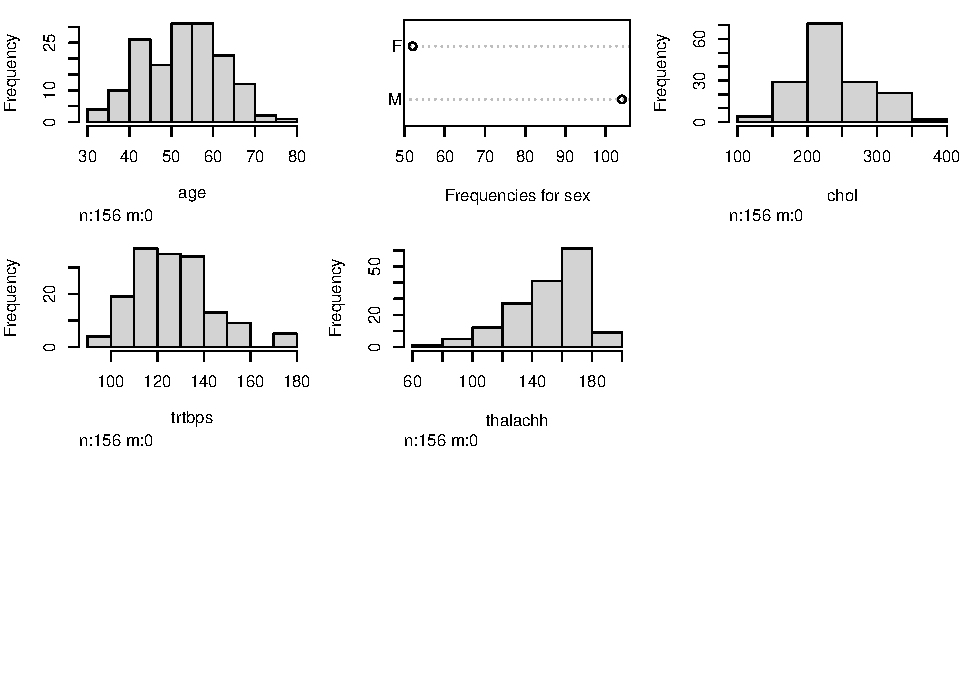
\includegraphics{PRA2_files/figure-latex/unnamed-chunk-10-1.pdf}

\begin{center}\rule{0.5\linewidth}{0.5pt}\end{center}

\hypertarget{anuxe1lisis-de-los-datos.}{%
\section{4 Análisis de los datos.}\label{anuxe1lisis-de-los-datos.}}

\hypertarget{selecciuxf3n-de-los-grupos-de-datos-que-se-quieren-analizarcomparar}{%
\subsection{4.1. Selección de los grupos de datos que se quieren
analizar/comparar}\label{selecciuxf3n-de-los-grupos-de-datos-que-se-quieren-analizarcomparar}}

\hypertarget{comprobaciuxf3n-de-la-normalidad-y-homogeneidad-de-la-varianza.}{%
\subsection{4.2. Comprobación de la normalidad y homogeneidad de la
varianza.}\label{comprobaciuxf3n-de-la-normalidad-y-homogeneidad-de-la-varianza.}}

\hypertarget{aplicaciuxf3n-de-pruebas-estaduxedsticas-para-comparar-los-grupos-de-datos.}{%
\subsection{4.3. Aplicación de pruebas estadísticas para comparar los
grupos de
datos.}\label{aplicaciuxf3n-de-pruebas-estaduxedsticas-para-comparar-los-grupos-de-datos.}}

Los datos que se van a utilizar en los siguientes análisis es el dataset
ya limpio de los anteriores apartados. Además, para cada análisis que se
modificará como sea necesario el dataframe.

\hypertarget{anuxe1lisis-de-correlaciones}{%
\subsubsection{Análisis de
correlaciones}\label{anuxe1lisis-de-correlaciones}}

\begin{verbatim}
## corrplot 0.92 loaded
\end{verbatim}

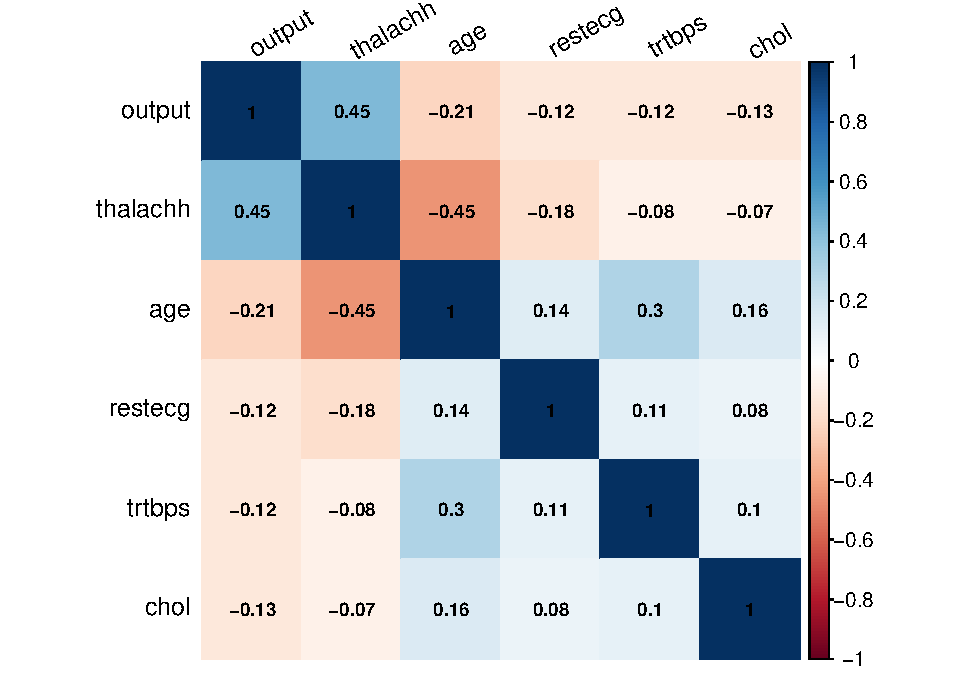
\includegraphics{PRA2_files/figure-latex/unnamed-chunk-11-1.pdf}

Se puede observar que hay una correlación moderada entre la variable
output (enfermedad cardíaca) y la variabla thalachh (frecuencia cardíaca
máxima alcanzada), ya que está llega a 0,45.

\hypertarget{anuxe1lisis-de-regresiuxf3n-loguxedstica}{%
\subsubsection{Análisis de regresión
logística}\label{anuxe1lisis-de-regresiuxf3n-loguxedstica}}

Una vez analizadas las correlaciones vamos a calcular la regresión
logística para calcular la variable de salida, la cual es dicotomica:

\begin{Shaded}
\begin{Highlighting}[]
\NormalTok{modelo }\OtherTok{\textless{}{-}} \FunctionTok{glm}\NormalTok{(dff}\SpecialCharTok{$}\NormalTok{output }\SpecialCharTok{\textasciitilde{}}\NormalTok{ dff}\SpecialCharTok{$}\NormalTok{age }\SpecialCharTok{+}\NormalTok{ dff}\SpecialCharTok{$}\NormalTok{sex }\SpecialCharTok{+}\NormalTok{ dff}\SpecialCharTok{$}\NormalTok{chol }\SpecialCharTok{+} 
\NormalTok{                dff}\SpecialCharTok{$}\NormalTok{restecg }\SpecialCharTok{+}\NormalTok{ dff}\SpecialCharTok{$}\NormalTok{trtbps }\SpecialCharTok{+}\NormalTok{ dff}\SpecialCharTok{$}\NormalTok{thalachh, }\AttributeTok{data=}\NormalTok{dff)}
\FunctionTok{summary}\NormalTok{(modelo)}
\end{Highlighting}
\end{Shaded}

\begin{verbatim}
## 
## Call:
## glm(formula = dff$output ~ dff$age + dff$sex + dff$chol + dff$restecg + 
##     dff$trtbps + dff$thalachh, data = dff)
## 
## Deviance Residuals: 
##     Min       1Q   Median       3Q      Max  
## -0.9764  -0.3459   0.1218   0.3206   0.8944  
## 
## Coefficients:
##                Estimate Std. Error t value Pr(>|t|)    
## (Intercept)   0.4078846  0.5267400   0.774 0.439947    
## dff$age      -0.0011712  0.0043163  -0.271 0.786509    
## dff$sexM     -0.2817279  0.0732739  -3.845 0.000178 ***
## dff$chol     -0.0010729  0.0007203  -1.490 0.138459    
## dff$restecg  -0.2143403  0.2191848  -0.978 0.329710    
## dff$trtbps   -0.0026384  0.0021204  -1.244 0.215335    
## dff$thalachh  0.0084627  0.0016328   5.183    7e-07 ***
## ---
## Signif. codes:  0 '***' 0.001 '**' 0.01 '*' 0.05 '.' 0.1 ' ' 1
## 
## (Dispersion parameter for gaussian family taken to be 0.1757739)
## 
##     Null deviance: 36.686  on 155  degrees of freedom
## Residual deviance: 26.190  on 149  degrees of freedom
## AIC: 180.33
## 
## Number of Fisher Scoring iterations: 2
\end{verbatim}

Tal y como se puede observar las variables más relevantes son el sexo y
el thalachh, ya que son las únicas que han resultado
significativas.\[(P_value < 0.05)\] Además, se cumple la estimación que
se había hecho en estudio de correlaciones, ya que la variable thalachh
tiene un impacto positivo, de forma que cuanto mayor sea, mayor es la
probabilidad de padecer una enfermedad cardiovascular.

\hypertarget{anuxe1lisis-de-contraste-de-hipuxf3tesis-de-dos-poblaciones}{%
\subsubsection{Análisis de contraste de hipótesis de dos
poblaciones}\label{anuxe1lisis-de-contraste-de-hipuxf3tesis-de-dos-poblaciones}}

Por último, se va a anlizar analizar si la edad media de los pacientes
es la misma independientemente del sexo. Es decir, se analizará si la
media de edad de los hombres y mujeres enfermos es la misma (output=1):

\begin{verbatim}
## Warning in leveneTest.default(y = y, group = group, ...): group coerced to
## factor.
\end{verbatim}

\begin{verbatim}
## Levene's Test for Homogeneity of Variance (center = median)
##       Df F value   Pr(>F)   
## group  1   8.097 0.005431 **
##       95                    
## ---
## Signif. codes:  0 '***' 0.001 '**' 0.01 '*' 0.05 '.' 0.1 ' ' 1
\end{verbatim}

\begin{verbatim}
## 
##  Shapiro-Wilk normality test
## 
## data:  dff_sick$age
## W = 0.97444, p-value = 0.055
\end{verbatim}

Gracias a estas pruebas se ha visto que aunque la varianza de esta
variable sea homogenea, es decir, y sigue una distribución normal. Ello
implica que podemos utilizar el contraste de hipótesis de medias usual:

\[
H_1: \mu_{m}\neq\mu_{f}\\
H_0: \mu_{m}=\mu_{f}
\]

En concreto, la prueba que se va a realizar es un contraste de hipótesis
bilateral:

\begin{Shaded}
\begin{Highlighting}[]
\CommentTok{\#Generamos dos grupos}
\NormalTok{dff1}\OtherTok{\textless{}{-}} \FunctionTok{subset}\NormalTok{(dff,dff}\SpecialCharTok{$}\NormalTok{output}\SpecialCharTok{==}\StringTok{\textquotesingle{}1\textquotesingle{}}\NormalTok{)}
\NormalTok{df\_m }\OtherTok{\textless{}{-}} \FunctionTok{subset}\NormalTok{(dff1,dff1}\SpecialCharTok{$}\NormalTok{sex }\SpecialCharTok{==} \StringTok{\textquotesingle{}M\textquotesingle{}}\NormalTok{)}
\NormalTok{df\_f }\OtherTok{\textless{}{-}} \FunctionTok{subset}\NormalTok{(dff1,dff1}\SpecialCharTok{$}\NormalTok{sex }\SpecialCharTok{==} \StringTok{\textquotesingle{}F\textquotesingle{}}\NormalTok{)}

\CommentTok{\#COmo no sigue una normal, hacemos uso del test Wilcox, }
\CommentTok{\#que analiza si las medianas de estos dos grupos son diferentes. }
\FunctionTok{t.test}\NormalTok{(df\_m}\SpecialCharTok{$}\NormalTok{age, df\_f}\SpecialCharTok{$}\NormalTok{age)}
\end{Highlighting}
\end{Shaded}

\begin{verbatim}
## 
##  Welch Two Sample t-test
## 
## data:  df_m$age and df_f$age
## t = -2.0762, df = 67.929, p-value = 0.04166
## alternative hypothesis: true difference in means is not equal to 0
## 95 percent confidence interval:
##  -8.3476793 -0.1653869
## sample estimates:
## mean of x mean of y 
##  49.76786  54.02439
\end{verbatim}

Como el \[ p-value\] sale menor a 0.05, se podría aceptar que hay
diferencia de edad media en entre las hombres enfermos con una
enfermedad cardiovascular y las mujeres.

\hypertarget{representaciuxf3n-de-los-resultados-a-partir-de-tablas-y-gruxe1ficas.}{%
\section{5. Representación de los resultados a partir de tablas y
gráficas.}\label{representaciuxf3n-de-los-resultados-a-partir-de-tablas-y-gruxe1ficas.}}

A lo largo de toda la práctica se han utilizado visualizaciones.

\hypertarget{resoluciuxf3n-del-problema.}{%
\section{6. Resolución del
problema.}\label{resoluciuxf3n-del-problema.}}

El problema presentado en un inicio era el análisis de los pacientes
enfermos de una enfermedad cardiovascular, a continuación se especifican
los resultados de dicho análisis:

Para empezar, se ha visto que la variable que más efecto tiene sobre la
variable dependiente, es thalachh, la frecuencia cardíaca máxima
alcanzada de las personas. Esto se ha podido ver tanto en el análisis de
correlaciones como en el modelo logístico.

Por otro lado, gracias al análisis de contrastes de media realizado se
ha podido concluir que la edad media de los hombres que padecen
enfermedades cardiovasculares es igual al de las mujeres, es decir, no
hay una significancia estadística.

\end{document}
